\section{Performance Evaluation}

We evaluated the performance of our code measuring runtime of our serial and
graph parallel code for a variety of $N$, $M$, and $T$. Additionally, we also
varied the number of cores available for Graphlab. R~\cite{r} was used for data
analysis and plotting. 

Our parallel code's runtime, compared to that of the serial version, is shown in
Figure~\ref{fig:runtime-256-500}. We see that, while our GraphLab implementation
runs slower than our serial implementation, the running time still decreases as
we increase the number of processing cores. 

\begin{figure*}[htb]
    \centering
    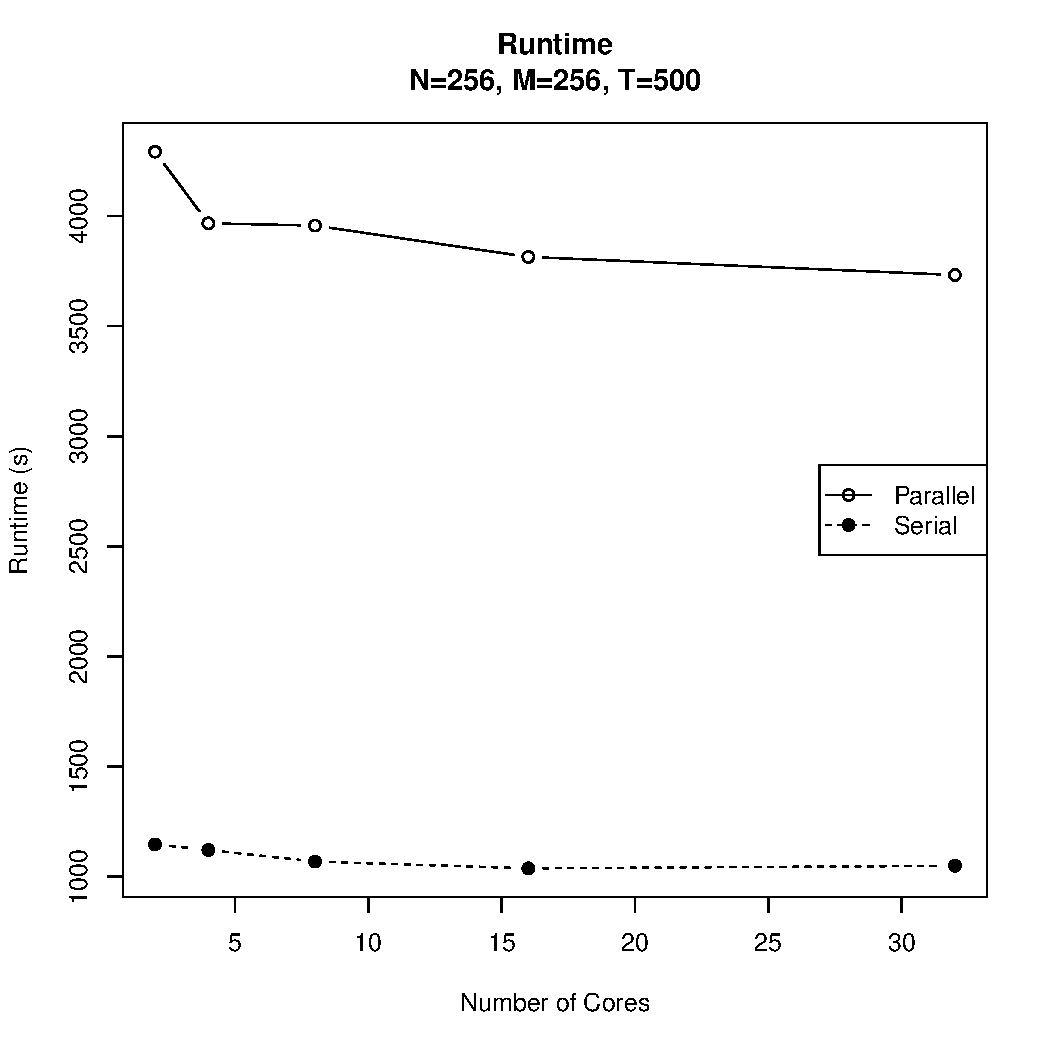
\includegraphics[width=0.6\textwidth]{../figure/runtime-N_256-T_500.pdf}
    \caption{Runtime as a function of number of cores used.}
    \label{fig:runtime-256-500}
\end{figure*}

Most compelling, we examined how our implementation scales as we increase the
problem size, especially $N$. A log-log plot of running time vs. $N$ is shown in
Figure~\ref{fig:scaling-16-200}. Judging by the slopes on the graph, our
GraphLab code scales better than the serial code, especially for smaller $N$. 

\begin{figure*}[htb]
    \centering
    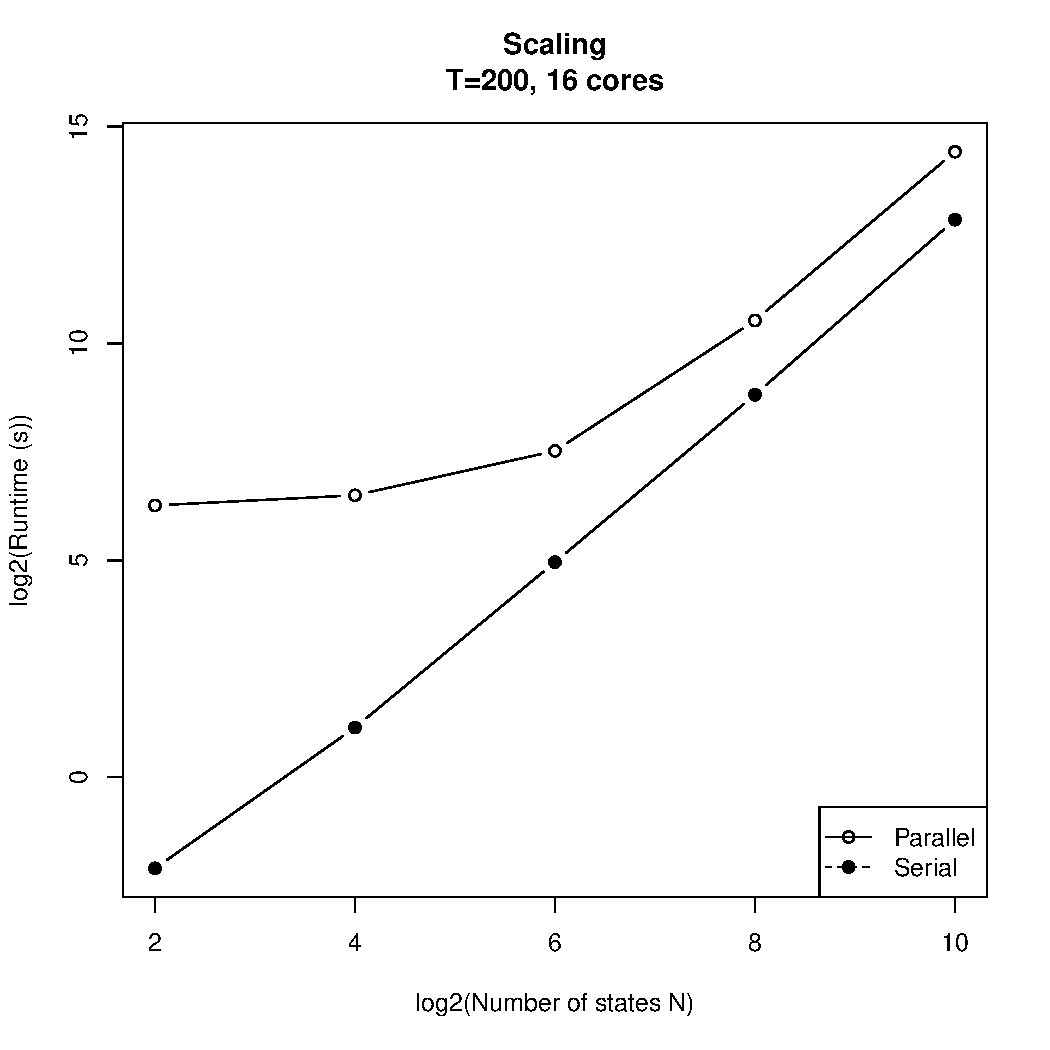
\includegraphics[width=0.6\textwidth]{../figure/scaling-cores_16-T_200.pdf}
    \caption{Log-Log plot of runtime as a function of number of states $N$.}
    \label{fig:scaling-16-200}
\end{figure*}
